\documentclass[11pt]{article}

\usepackage{amsmath}
\usepackage{amsfonts}
\usepackage{amssymb}
\usepackage{graphicx}
\usepackage{tikz}
\usepackage{pgfplots}
\usepackage{authblk}
\usepackage{url}
\usepackage{hyperref}

\pgfplotsset{compat=1.17}

\title{Spectral Graph Coagulation and the Emergence of Hybrid Discrete Geometry}
\author{Eduardo Gonzalez-Granda Fernandez\\
\textit{Independent Researcher, Salamanca, Spain}\\
\href{mailto:eggranda@usal.es}{eggranda@usal.es}\\
\href{https://orcid.org/0000-0002-6771-5145}{ORCID: 0000-0002-6771-5145}
%10.5281/zenodo.19038286
}
\date{\today \\ \vspace{0.4cm} 
\textbf{DOI:} \href{https://doi.org/10.5281/zenodo.xxx}{10.5281/zenodo.19038286}}

\begin{document}

\maketitle

\begin{abstract}
We introduce a dynamical model of graph aggregation governed by spectral compatibility between discrete clusters.
In the model, connected graphs merge through pairwise fusion events whose acceptance depends on Laplacian-based observables, including eigenvalue dispersion, inverse participation ratio, and spectral gap.
Although the microscopic rule is purely combinatorial and does not assume any background geometry, the resulting graph-soup dynamics generates highly structured large-scale networks.

At coarse-grained level, the merger statistics are well described by an effective coagulation kernel
\[
K(i,j)\sim (ij)^\gamma,
\qquad
\gamma \approx 0.66,
\]
placing the system in a sub-multiplicative aggregation regime.
More importantly, the resulting networks do not merely form a giant component.
They remain sparse while developing extensive loop topology, with first Betti number scaling approximately as
\[
\beta_1 \sim N^{1.1768}.
\]

Geometric analysis reveals the emergence of a hybrid discrete geometry.
The growth of graph-metric balls follows a power law compatible with an effective metric dimension
\[
N(r)\sim r^{d_f},
\qquad
d_f \approx 3.4,
\]
while the spectral dimension extracted from random-walk return probabilities reaches an approximately stationary large-scale regime
\[
d_s = 3.12 \pm 0.40
\]
for clusters with $N>5000$.
At the same time, the graph ensemble exhibits persistently negative Forman curvature and compressed global distances, indicating that the emergent structure is locally finite-dimensional but globally hyperbolic-like.

We also find that the dominant eigenmode is extended rather than hub-dominated, showing that the spectral radius is controlled by collective structural organization rather than by isolated high-degree vertices.
Taken together, these results show that spectrally selective coagulation generates sparse, loop-rich, negatively curved graph ensembles with stable large-scale diffusion dimension close to three.

More broadly, the model provides a minimal framework in which topology, dimension, curvature, and large-scale organization emerge jointly from purely relational graph dynamics, with possible relevance both for structured network formation and for toy models of emergent discrete geometry.
\end{abstract}
\section{Introduction}

Understanding how geometric structure can emerge from purely combinatorial
or relational systems is a central problem across multiple areas of physics,
mathematics, and complex systems science. In particular, the question of
whether notions such as dimension, curvature, and spatial organization can
arise from simple interaction rules on discrete structures remains largely open.

Graph-based models provide a natural framework to explore this problem.
They encode relational information without assuming any underlying geometry,
making them ideal candidates for studying the emergence of effective spatial
properties. In recent years, various approaches have investigated how
geometric features can arise in networks, including models of network geometry,
random simplicial complexes, and approaches inspired by quantum gravity.

A key insight from these studies is that geometry may not be a fundamental
ingredient, but rather an emergent property resulting from dynamical constraints.
In this context, spectral properties of graphs — particularly those related
to the eigenvalues and eigenvectors of adjacency or Laplacian operators —
play a central role. The spectral radius, in particular, encodes global
connectivity and stability properties of the network.

In this work, we introduce and study a simple yet non-trivial dynamical model
of graph growth, which we refer to as \emph{spectral coagulation}. In this model,
graphs grow through successive fusion events governed by a spectral stability
criterion. Specifically, the merging of graph components is constrained by
their effect on the spectral radius of the resulting structure.

The central question we address is the following:

\begin{quote}
\emph{Can a local rule based solely on spectral stability generate networks
with non-trivial topology and well-defined geometric properties?}
\end{quote}

Through extensive numerical simulations and systematic analysis, we show that
the answer is affirmative. The dynamics leads to the spontaneous emergence of
networks with the following properties:

\begin{itemize}
    \item A non-trivial topological structure characterized by a number of
    independent cycles scaling linearly with system size.

    \item An effective geometric organization with volume scaling
    $N(r) \sim r^{d_f}$, where $d_f \approx 3.4$.

    \item A spectral dimension $d_s = 3.12 \pm 0.40$, indicating diffusion properties
    consistent with a three-dimensional structure.

    \item A dominant eigenmode that is not localized on hubs but extended
    across the network, reflecting collective organization.

    \item A persistent negative Forman curvature, indicating global
    hyperbolic features.

\end{itemize}

Taken together, these results reveal the emergence of a \emph{hybrid geometry}:
the network behaves locally as a three-dimensional space, while globally
exhibiting features associated with negative curvature and long-range
connectivity.

Importantly, these properties arise without imposing any geometric constraints
a priori. The only guiding principle is a local rule based on spectral stability.
This suggests that spectral constraints may act as a fundamental organizing
principle capable of generating both topology and geometry in complex systems.

Beyond their intrinsic theoretical interest, these results have potential
implications in several domains. In network science, they provide a mechanism
for generating structured networks with controlled spectral properties.
In statistical physics, they offer insight into self-organized systems with
emergent geometry. More speculatively, they may inform approaches to emergent
space-time in discrete models of quantum gravity, where geometry is expected
to arise from underlying combinatorial structures.

The paper is organized as follows. In Section~\ref{sec:model}, we define the
spectral coagulation model. Section~\ref{sec:methods} describes the simulation
and analysis methods. Sections~\ref{sec:topology}–\ref{sec:curvature} present
the results on topology, geometry, spectral structure, and curvature.
Finally, Section~\ref{sec:discussion} discusses the implications of the model,
and Section~\ref{sec:conclusion} summarizes the main findings.
\section{Spectral Graph Coagulation Model}

We consider a dynamical system consisting of a population of graphs that merge through pairwise fusion events.
Each graph represents a connected component whose internal structure evolves only through aggregation with other graphs.
The aim of the model is to test whether a local rule based on spectral compatibility can generate large-scale topological and geometric order.

\subsection{Graph Representation}

Each cluster is represented by a finite, simple, undirected graph
\[
G = (V,E),
\]
where $V$ is the set of vertices and $E$ the set of edges.
The size of a graph is defined as
\[
n = |V|.
\]

Two matrix representations play a central role in the analysis.

First, the adjacency matrix $A$ is defined by
\[
A_{ij}=
\begin{cases}
1,& \text{if } (i,j)\in E,\\
0,& \text{otherwise}.
\end{cases}
\]
Its dominant eigenvalue controls the leading collective connectivity mode of the graph.

Second, the graph Laplacian is
\[
L = D - A,
\]
where $D$ is the diagonal degree matrix.
The Laplacian spectrum
\[
0 = \lambda_1 \le \lambda_2 \le \dots \le \lambda_n
\]
encodes structural information about the network, including connectivity, diffusion, and effective dimensionality.

Throughout the paper we use the adjacency spectrum mainly to characterize the dominant collective mode and the Laplacian spectrum to probe diffusion, spectral dimension, and geometric structure.

\subsection{Spectral Observables}

To characterize each graph we compute several observables derived from the adjacency or Laplacian spectrum.

\paragraph{Eigenvalue dispersion.}
For the Laplacian spectrum we define the eigenvalue dispersion
\[
\sigma(G) = \sqrt{\frac{1}{n}\sum_{k=1}^{n} (\lambda_k-\bar{\lambda})^2},
\]
where
\[
\bar{\lambda}=\frac{1}{n}\sum_{k=1}^{n}\lambda_k
\]
is the mean Laplacian eigenvalue.

\paragraph{Inverse participation ratio.}
To quantify localization properties of eigenvectors we compute the inverse participation ratio (IPR)
\[
\mathrm{IPR}(v) = \sum_i |v_i|^4,
\]
where $v$ is a normalized eigenvector.
For a perfectly delocalized mode one has $\mathrm{IPR}\sim 1/n$, whereas for a strongly localized mode the IPR remains finite as $n$ grows.

\paragraph{Spectral gap.}
The Laplacian spectral gap is
\[
\Delta = \lambda_2-\lambda_1 = \lambda_2,
\]
since $\lambda_1=0$ for a connected graph.
This quantity provides information about connectivity, expansion, and diffusion time scales.

\paragraph{Dominant adjacency eigenvalue.}
In addition to Laplacian observables, we denote by
\[
\Lambda_1(A)
\]
the largest eigenvalue of the adjacency matrix.
This quantity will play an important role in the later analysis, since the numerical simulations show that the global organization of the graph soup is strongly constrained by the behavior of this dominant spectral mode.

\subsection{Fusion Dynamics as Spectral Compatibility}

At each step of the dynamics two graphs $G_i$ and $G_j$ are selected from the population.
A tentative fusion event is proposed by joining the two graphs through a set of interconnections.
Whether this fusion is accepted depends on a spectral compatibility criterion.

A convenient phenomenological way to express this idea is through a relational mismatch energy $E_{ij}$ built from differences in spectral observables between the two parent graphs. For example, one may define
\[
\Delta \sigma = |\sigma(G_i)-\sigma(G_j)|,
\]
\[
\Delta \mathrm{IPR} = |\mathrm{IPR}(G_i)-\mathrm{IPR}(G_j)|,
\]
\[
\Delta \Delta = |\Delta(G_i)-\Delta(G_j)|.
\]
A generic linear combination is then
\[
E_{ij} = k_\sigma \Delta\sigma + k_{\mathrm{ipr}} \Delta\mathrm{IPR} + k_{\mathrm{gap}} \Delta\Delta,
\]
where $k_\sigma$, $k_{\mathrm{ipr}}$, and $k_{\mathrm{gap}}$ are effective couplings.

In some implementations this mismatch may be converted into an acceptance probability of Boltzmann type,
\[
P_{ij} = \exp\!\left(-\frac{E_{ij}}{T}\right),
\]
with $T$ an effective temperature.
However, for the purposes of the present paper the essential point is more general:
fusion is not purely random, but spectrally selective.
The dynamics favors mergers that preserve or enhance collective spectral coherence while disfavoring strongly incompatible combinations.

\begin{figure}[t]
\centering

\includegraphics[width=0.9\linewidth]{images/fig_spectral_mechanism.pdf}
\caption{Spectral mechanism underlying the aggregation dynamics. Two clusters fuse through a set of interconnections, thereby modifying the dominant collective mode of the combined graph. The acceptance of the merger is controlled by spectral compatibility.}
\end{figure}

\subsection{Graph Fusion}

When a fusion event is accepted, the two graphs are merged into a single graph
\[
G = G_i \cup G_j.
\]

More precisely, if $G_i=(V_i,E_i)$ and $G_j=(V_j,E_j)$ are disjoint, the fused graph is
\[
G = (V_i\cup V_j,\; E_i\cup E_j\cup E_{\mathrm{bridge}}),
\]
where $E_{\mathrm{bridge}}$ is the set of newly introduced interconnections between the two components.

If the number of such interconnections is denoted by $m$, then the fused graph has
\[
n = n_i+n_j
\]
vertices and
\[
|E| = |E_i|+|E_j|+m
\]
edges.

In the numerical simulations studied in this paper, the number of interconnections is not merely of order unity.
Rather, it scales approximately with the size of the smaller cluster,
\[
m \sim \min(i,j),
\]
which is a crucial structural ingredient of the model.
This implies that fusion events typically create not only connectivity between components, but also a substantial number of new cycles and long-range shortcuts.

\subsection{Population Dynamics}

The system evolves through repeated fusion events until no further mergers are possible or until the population of graphs becomes exhausted.

During the evolution we record:
\begin{itemize}
\item cluster sizes,
\item spectral observables,
\item fusion events,
\item topological and geometric graph properties.
\end{itemize}

These data allow us to reconstruct the effective large-scale behavior of the coagulation process and to analyze the structure of the resulting large clusters.

\subsection{Spectral Origin of the Aggregation Mechanism}

To understand the origin of the effective aggregation mechanism we consider the spectral properties of the fused graph formed by joining two clusters of sizes $i$ and $j$.

Let $A_i$ and $A_j$ denote the adjacency matrices of the two clusters.
The adjacency matrix of the combined system can be written as
\[
A =
\begin{pmatrix}
A_i & B \\
B^{T} & A_j
\end{pmatrix},
\]
where the matrix $B$ represents the set of interconnections created between the two graphs.

The dominant adjacency eigenvalue $\Lambda_1$ determines the leading collective mode of the network.
When two graphs are connected, the shift in this mode may be estimated heuristically using spectral perturbation theory.
If $v$ denotes the dominant eigenvector of the uncoupled block matrix, the leading correction has the form
\[
\delta \Lambda_1 \approx \frac{v^{T} P v}{v^{T}v},
\]
where $P$ is the perturbation induced by the bridging block.

The magnitude of this correction depends on two competing effects:

\begin{enumerate}
\item the number of newly created interconnections, encoded in $B$,
\item the degree of localization or delocalization of the dominant mode.
\end{enumerate}

If the number of bridging edges scales as
\[
m \sim \min(i,j),
\]
then the spectral norm of the perturbation matrix typically grows with $m$.
At the same time, numerical analysis shows that the dominant eigenmode is not localized on a few hubs but distributed over a substantial fraction of the graph.
Therefore the spectral response to fusion is collective rather than hub-dominated.

This point is important: the leading spectral mode of the graph soup is not controlled by isolated nodes of exceptionally high degree, but by the global architecture of the fused network.
As a result, spectral selection acts as a genuinely collective constraint on graph growth.

\subsection{Topological Effect of Fusion}

The addition of bridging edges has an immediate topological consequence.
If two connected graphs are joined by $m$ interconnections, the first one is sufficient to connect the two components, while each additional one creates an independent cycle.
Thus the first Betti number
\[
\beta_1 = |E|-|V|+C
\]
increases approximately as
\[
\Delta \beta_1 \approx m-1.
\]

Since $m$ scales approximately with the size of the smaller cluster, repeated fusion events generate an extensive number of cycles.
This heuristic expectation is fully consistent with the numerical results reported later, where we find
\[
\beta_1 \propto N^\alpha,
\qquad \alpha \approx 1.18,
\]
that is, an almost linear growth of topological complexity with system size.

\subsection{Spectral-Dimension Interpretation}

An alternative and complementary way to understand the aggregation dynamics is through the concept of spectral dimension.
This viewpoint is particularly natural when the graph is regarded as an emergent discrete geometry.

\paragraph{Diffusion and spectral dimension.}

For a graph Laplacian $L$, diffusion processes obey
\[
\partial_t p = -Lp.
\]
The return probability of a random walk behaves asymptotically as
\[
P(t)\sim t^{-d_s/2},
\]
where $d_s$ is the spectral dimension.

This quantity characterizes the effective dimensionality probed by diffusion.
It can also be extracted from the low-eigenvalue density of states, which for a graph of spectral dimension $d_s$ satisfies
\[
\rho(\lambda)\sim \lambda^{d_s/2-1}.
\]

The numerical analysis performed in this work shows that large clusters produced by the coagulation dynamics approach
\[
d_s = 3.12 \pm 0.40.
\]
This result is obtained consistently from random-walk estimates and from the scaling of the spectral density, including a finite-size spectral collapse.
The value $d_s\approx 3$ is therefore not an accidental feature of one particular estimator, but an intrinsic property of the graph ensemble.

\begin{figure}[t]
\centering

\includegraphics[width=8cm]{images/fig_spectral_dimension_vs_size.pdf}
\caption{
Spectral dimension of clusters generated in the graph-soup simulation as a function of cluster size.
Small clusters display broad fluctuations and lower effective dimensionality, while larger clusters tend toward a stable value close to $d_s = 3.12 \pm 0.40$.
This convergence is consistent with the spectral density analysis presented later and indicates the emergence of an effective three-dimensional diffusion geometry at large scales.
}
\label{fig:dimension_vs_cluster_size}
\end{figure}

\paragraph{Scaling of Laplacian eigenvalues.}

If the low-lying Laplacian density of states obeys
\[
\rho(\lambda)\sim \lambda^{d_s/2-1},
\]
then the cumulative mode count scales as
\[
N_\lambda \sim N\,\lambda^{d_s/2}.
\]
From this one infers the characteristic finite-size scaling of low eigenvalues,
\[
\lambda \sim N^{-2/d_s}.
\]
For $d_s\approx 3$, this gives
\[
\lambda \sim N^{-2/3}.
\]

This relation is important because it links spectral spacing directly to effective dimensionality.

\paragraph{Fusion of two graphs.}

Consider now the fusion of two clusters of sizes $i$ and $j$.
The final graph contains
\[
N=i+j
\]
vertices plus a set of bridging edges.
These links hybridize diffusion modes originally supported on the two components.

At a heuristic level, the characteristic spectral perturbation induced by fusion depends on two ingredients:
\begin{itemize}
\item the abundance of coupling channels between the two components,
\item the finite-size spacing of low diffusion modes.
\end{itemize}

Since the number of interconnections grows with $\min(i,j)$ and the low-mode spacing scales as $N^{-2/d_s}$, one expects the spectral effect of fusion to depend both on cluster size and on the emergent spectral dimension.

\paragraph{Interpretive consequence.}

The key point is not a single exact power-law kernel, but rather the following:
because the spectral dimension approaches $d_s\approx 3$, the low-frequency sector of the graph behaves as that of an effective three-dimensional discrete medium.
At the same time, the later curvature analysis will show that the global organization is not purely Euclidean, but carries persistent negative curvature.

Thus the graph soup does not simply generate a random network.
It produces a hybrid geometry: locally diffusion behaves as in an approximately three-dimensional structure, while globally the network exhibits long-range organization and hyperbolic-like curvature.

\paragraph{Relation to discrete quantum geometry.}

The appearance of spectral dimension is particularly intriguing because it plays a central role in several approaches to quantum gravity based on discrete structures.
In such settings, geometry is not fundamental but encoded in spectral and combinatorial observables.

From this perspective, the aggregation dynamics studied here can be interpreted as a form of relational graph growth in which effective geometric properties emerge from spectral interactions between discrete building blocks.
We do not claim that the model is a theory of space-time.
However, the coexistence of an effective dimension, non-trivial curvature, and collective spectral modes makes it a useful toy model for studying how geometry may emerge from purely relational dynamics.
\section{Numerical Results}

\begin{figure}[t]
\centering

\includegraphics[width=8cm]{images/kcore_structure_final.pdf}
\caption{
Structure of a large connected component produced by spectral graph coagulation.
Nodes belonging to the $3$-core are shown in red, while peripheral nodes are shown in gray.
The network exhibits a clear backbone-plus-periphery organization, with a large fraction of nodes belonging to a connected structural core.
}
\label{fig:core_structure}
\end{figure}

We performed extensive numerical simulations of the spectral graph coagulation model described in the previous section.
The system was initialized with a population of small connected graphs generated from the atomic database \cite{gonzalez2025algebraic} and evolved through repeated fusion events according to a spectrally selective acceptance rule.

Throughout the simulations we recorded cluster sizes, spectral observables, and structural properties of the resulting graphs.
These measurements allow us to characterize both the aggregation dynamics and the emergent topology and geometry of the large connected components.

\subsection{Growth of the Giant Component}

A central observable of the system is the size of the largest connected component as a function of fusion events.
In all simulations we observe the rapid emergence of a dominant cluster that absorbs most of the nodes in the system.

After an initial transient regime, the largest connected component grows steadily until the available population of smaller graphs becomes depleted.
This behavior is consistent with a coagulation process in which repeated mergers progressively concentrate mass into a giant cluster.

\subsection{Large-Scale Structural Organization}

The networks produced by the aggregation dynamics are sparse but highly organized.
Although the number of nodes grows over several orders of magnitude, the average degree remains relatively low, typically in the range
\[
\langle k\rangle \sim 3\text{--}6.
\]
At the same time, the resulting graphs do not resemble trees or locally trivial sparse networks.
Instead, they develop a non-trivial backbone with abundant cycles and a pronounced core-plus-periphery architecture.

This feature is already visible in the $k$-core structure shown in Fig.~\ref{fig:core_structure}.
A large fraction of the network belongs to a non-trivial core, while the remaining nodes form a peripheral region attached to this backbone.
The existence of such a core is consistent with the later topological analysis, which shows that the number of independent cycles grows approximately linearly with system size.

\subsection{k-core Structure}

To characterize the internal organization of the giant component we perform a $k$-core decomposition.

The $k$-core of a graph is the maximal induced subgraph in which all vertices have degree at least $k$.
The decomposition reveals a robust backbone corresponding typically to the $3$-core of the network.

In the simulated graph ensemble, the $3$-core often contains a substantial fraction of the nodes in the giant component, typically between $60\%$ and $80\%$ depending on graph size and realization.
This result indicates that the large connected clusters are not merely tenuous sparse aggregates, but possess a structurally cohesive interior.

Empirically, the maximal nontrivial core index is of the same order as the mean degree,
\[
k_{\mathrm{core}}^{\max} \sim \lfloor \langle k\rangle \rfloor,
\]
which is natural for sparse networks with an organized but not hub-dominated backbone.

\subsection{Effective Coagulation Behavior}

To characterize the aggregation process one may measure the frequency of fusion events between clusters of size $i$ and $j$ and construct an effective coagulation kernel
\[
K(i,j).
\]

Over the accessible range of sizes, the measured kernel can be approximated by a power-law form
\[
K(i,j)\sim (ij)^{\gamma}
\]
with an effective exponent close to
\[
\gamma \approx 0.66.
\]

However, this exponent should not be interpreted as a universal asymptotic law.
The simulations indicate that the graph ensemble undergoes substantial structural evolution with cluster size, including changes in spectral dimension, topology, and global organization.
The measured kernel exponent is therefore best regarded as an effective finite-range descriptor of the aggregation dynamics rather than as a fundamental scaling law.

\begin{figure}[t]
\centering

\includegraphics[width=0.85\linewidth]{images/fig_kernel_scaling.pdf}
\caption{Measured coagulation kernel $K(i,j)$ versus product $ij$ on a log-log scale. Points represent binned data; the red line shows a linear fit with effective slope $\gamma \approx 0.66$. This fit is useful as a finite-range phenomenological description, although later results show that the graph ensemble develops nontrivial geometry and does not obey a single homogeneous scaling law at all scales.}
\label{fig:kernel}
\end{figure}

\subsection{From Sparse Growth to Emergent Geometry}

At a purely combinatorial level, one might expect repeated fusion of sparse graphs to produce either tree-like structures or heterogeneous hub-dominated networks.
The numerical results show that neither of these scenarios is realized.

Instead, the coagulation process generates networks with the following simultaneous properties:

\begin{itemize}
\item low mean degree,
\item a large non-trivial $k$-core,
\item an extensive number of independent cycles,
\item short path lengths,
\item a well-defined effective spectral dimension.
\end{itemize}

These features strongly suggest that the graph soup is self-organizing into a geometrically nontrivial state rather than a generic random sparse graph.
The later sections will show that this state combines local three-dimensional diffusion properties with global negative curvature.

\subsection{Summary of the Numerical Regime}

The main conclusion of the simulations reported in this section is that spectral coagulation robustly produces large connected networks with a stable structural backbone.
The graph ensemble remains sparse, but its organization is far from trivial:
the large clusters display a core-periphery structure, persistent cycle formation, and signatures of emergent geometry.

\begin{figure*}[t]
\centering
\begin{tabular}{cc}

% PANEL A
\begin{tikzpicture}
\begin{axis}[
width=6cm,
height=5cm,
xlabel={Fusion events},
ylabel={Largest component size},
title={A. Giant component growth}
]
\addplot[blue, thick] table {data/giant_component.dat};
\end{axis}
\end{tikzpicture}

&

% PANEL B
\begin{tikzpicture}
\begin{axis}[
width=6cm,
height=5cm,
xlabel={$\log(ij)$},
ylabel={$\log K(i,j)$},
title={B. Effective coagulation kernel}
]
\addplot[only marks] table {data/kernel_points.dat};
\addplot[red, thick] table {data/kernel_fit.dat};
\end{axis}
\end{tikzpicture}

\\

% PANEL C
\begin{tikzpicture}
\begin{axis}[
width=6cm,
height=5cm,
xlabel={$k$},
ylabel={Fraction of nodes},
title={C. $k$-core structure}
]
\addplot[ybar] table {data/kcore_distribution.dat};
\end{axis}
\end{tikzpicture}

&

% PANEL D
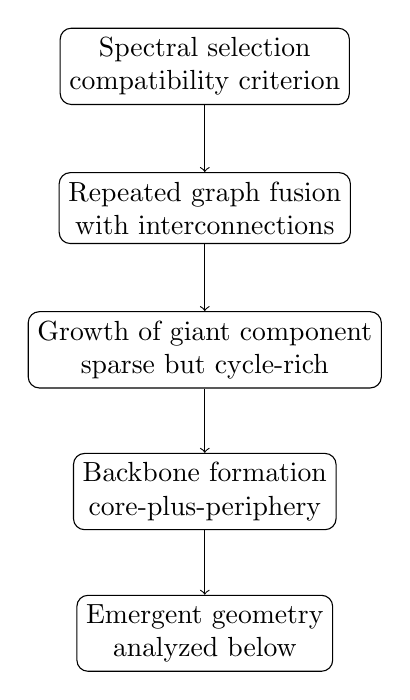
\begin{tikzpicture}[
node distance=1.8cm,
box/.style={rectangle,draw,rounded corners,align=center}
]

\node[box] (spectral) {Spectral selection \\ compatibility criterion};
\node[box, below of=spectral] (fusion) {Repeated graph fusion \\ with interconnections};
\node[box, below of=fusion] (growth) {Growth of giant component \\ sparse but cycle-rich};
\node[box, below of=growth] (structure) {Backbone formation \\ core-plus-periphery};
\node[box, below of=structure] (geometry) {Emergent geometry \\ analyzed below};

\draw[->] (spectral) -- (fusion);
\draw[->] (fusion) -- (growth);
\draw[->] (growth) -- (structure);
\draw[->] (structure) -- (geometry);

\end{tikzpicture}

\end{tabular}

\caption{
Emergence of large-scale organization from spectral graph coagulation.
(A) Growth of the giant component during fusion dynamics.
(B) Effective coagulation kernel measured over the accessible size range.
(C) $k$-core decomposition revealing a dominant structural backbone.
(D) Conceptual scheme linking spectral selection, repeated fusion, backbone formation, and emergent geometry.
}
\label{fig:summary}
\end{figure*}
\section{Core Structure and Mean-Degree Constraint}

One of the most robust empirical observations in the simulations is the relation between the maximal non-trivial $k$-core index and the mean degree of the network.

Across a broad range of realizations we observe that
\[
k_{\mathrm{core}}^{\max}
\]
is of the same order as
\[
\lfloor \langle k\rangle \rfloor .
\]

In the large connected clusters generated by the spectral coagulation dynamics, the mean degree typically remains in the range
\[
\langle k\rangle \sim 3\text{--}6,
\]
and the dominant non-trivial core is very often the $3$-core.
This suggests that the structural backbone of the graph is strongly constrained by the global edge density.

\subsection{A global constraint from degree balance}

Let $N$ be the number of nodes and $E$ the number of edges in a connected graph.
The mean degree is
\[
\langle k\rangle = \frac{2E}{N}.
\]

Suppose that the network contains a $k$-core of size $N_c$.
By definition, every node in this core has degree at least $k$, so the sum of degrees over the core satisfies
\[
\sum_{i\in\mathrm{core}} k_i \ge kN_c.
\]

On the other hand, the total degree sum over the whole graph is fixed by
\[
\sum_i k_i = N\langle k\rangle.
\]

Therefore one necessarily has
\[
kN_c \le N\langle k\rangle,
\]
or equivalently,
\[
k \le \langle k\rangle \frac{N}{N_c}.
\]

This inequality is elementary but informative: a large dense core can only exist if the global mean degree is sufficiently large to support it.

\subsection{Large-core regime}

In the graph soup produced by spectral coagulation, the giant component typically contains a structurally significant backbone occupying a finite fraction of the graph,
\[
N_c \approx \alpha N,
\]
with
\[
\alpha \sim 0.6\text{--}0.8
\]
in typical realizations.

Substituting into the previous inequality gives
\[
k \le \frac{\langle k\rangle}{\alpha}.
\]

Since $\alpha$ is of order unity, this implies that the maximal core index cannot exceed the mean degree by more than a moderate factor.
For example, if $\langle k\rangle \approx 3.3$ and $\alpha \approx 0.7$, one obtains the bound
\[
k \lesssim 4.7.
\]

Thus, in sparse graphs whose dense backbone occupies a substantial fraction of the nodes, one naturally expects the maximal non-trivial $k$-core to be of the same order as the mean degree, rather than parametrically larger.

\subsection{Interpretation of the observed 3-core}

The numerical simulations consistently show the emergence of a dominant $3$-core backbone.
This is fully compatible with the degree-balance argument above.

The point is not that degree conservation alone forces
\[
k_{\mathrm{core}}^{\max} = \lfloor \langle k\rangle \rfloor
\]
as an exact identity.
Rather, the argument shows that once the graph remains sparse and the backbone occupies a finite fraction of the system, only relatively low core indices are globally sustainable.
In this regime, a robust $3$-core is the natural structural outcome for networks with mean degree of order three or slightly above.

\subsection{Consequences for spectral coagulation}

This observation helps explain why the backbone structure is stable across realizations.
The spectral coagulation dynamics generates large graphs with low mean degree but non-trivial cycle density.
Such networks are sparse enough to exclude very high-order cores, yet sufficiently interconnected to sustain a macroscopic $3$-core.

Therefore the emergence of the backbone is not a superficial visual feature but a structural consequence of the coexistence of two constraints:

\begin{itemize}
\item low global edge density,
\item extensive topological complexity generated by repeated fusion events.
\end{itemize}

In this sense, the dominant core structure provides an intermediate signature between purely local degree information and the more global topological and geometric observables analyzed in the following sections.
\section{Continuum Description of the Aggregation Dynamics}

The numerical results presented above suggest that, at a coarse-grained level, the large-scale evolution of the graph soup can be described as an aggregation process between clusters.
At sufficiently large scales, the detailed spectral rules governing individual fusion events may be replaced by an effective kinetic description in terms of cluster-size distributions.

This continuum viewpoint is useful as a phenomenological description of mass transfer across scales.
However, it should be emphasized from the outset that it does not capture the full geometric content of the model.
The later sections will show that the graph ensemble develops non-trivial topology, effective dimension, collective spectral modes, and negative curvature.
Thus the continuum coagulation picture is informative, but only partial.

\subsection{Cluster Size Distribution}

Let $c(n,t)$ denote the concentration of clusters containing $n$ nodes at time $t$.
The evolution of this distribution under binary fusion events can be modeled by the Smoluchowski coagulation equation
\[
\frac{\partial c(n,t)}{\partial t}
=
\frac12
\sum_{i+j=n}
K(i,j)c(i,t)c(j,t)
-
c(n,t)\sum_j K(n,j)c(j,t),
\]
where $K(i,j)$ is an effective coagulation kernel describing the rate at which clusters of size $i$ and $j$ merge.

In the present context, this equation should be interpreted as a mesoscopic approximation to the underlying graph dynamics.
The exact microscopic rule is not a direct size-based merger probability, but a spectrally selective fusion criterion acting on the internal structure of the graphs.
The kernel $K(i,j)$ therefore summarizes, in an averaged way, the combined effect of size, spectral compatibility, and internal connectivity.

\subsection{Effective Coagulation Kernel}

From the recorded fusion events in the simulations one may estimate an effective kernel by measuring the frequency of mergers between clusters of size $i$ and $j$ and correcting for the population of available clusters of each size.

Over the accessible range of sizes, the data are reasonably approximated by
\[
K(i,j)\sim (ij)^{\gamma},
\]
with an effective exponent
\[
\gamma \approx 0.66.
\]

This scaling is useful as a finite-range empirical summary of the aggregation kinetics.
However, it should not be interpreted as a universal asymptotic law.
The structural properties of the clusters evolve significantly with size, and later analyses will show that the graph ensemble develops non-trivial geometric features.
Accordingly, the measured exponent is best viewed as an effective descriptor of the observed regime rather than as a fundamental parameter of the model.

\subsection{Formation of a Giant Component}

A standard implication of coagulation dynamics is the progressive transfer of mass toward larger clusters.
This is indeed what is observed numerically: after an initial transient, a dominant connected component rapidly emerges and then absorbs a large fraction of the total number of nodes.

From the continuum perspective, this behavior is consistent with an aggregation process in which merger rates increase with cluster size over the sampled range.
In this sense, the effective Smoluchowski picture captures one essential feature of the simulations: the concentration of mass into a giant component.

At the same time, the graph-theoretic structure of the emerging component is far more constrained than in generic coagulation models.
The resulting cluster is not simply a large aggregate characterized only by its mass, but a sparse network with organized topology and geometry.

\subsection{Sparse Growth Regime}

Despite the continuous growth of the giant component, the resulting graphs remain sparse.
If $N$ denotes the number of nodes and $E$ the number of edges, the mean degree is
\[
\langle k\rangle = \frac{2E}{N}.
\]

The numerical simulations show that $\langle k\rangle$ remains low throughout the growth process, typically in the range
\[
\langle k\rangle \sim 3\text{--}6.
\]

Thus, although the clusters become very large, the number of edges grows only linearly with the number of nodes.
This places the system in a sparse regime.

This fact is structurally important.
It implies that the graph soup does not evolve toward dense random graphs.
Instead, it grows as a sparse but highly organized network in which the addition of edges is constrained by the spectral selection rule.
Later sections will show that this sparse regime coexists with extensive cycle formation, a non-trivial core structure, effective three-dimensional diffusion, and negative curvature.

\subsection{Limits of the Continuum Picture}

The continuum description in terms of $c(n,t)$ and $K(i,j)$ is useful for describing coarse mass redistribution across cluster sizes, but it necessarily discards most of the internal graph structure.

In particular, the Smoluchowski equation does not track:

\begin{itemize}
\item the number of independent cycles,
\item the $k$-core structure,
\item distance scaling,
\item spectral dimension,
\item localization properties of the dominant eigenmode,
\item discrete curvature.
\end{itemize}

These observables are not secondary details; they are precisely the quantities that reveal the emergent geometry of the graph soup.
Therefore the continuum aggregation model should be regarded as a reduced kinetic description, valid at the level of cluster sizes but insufficient to characterize the full large-scale organization of the networks.

\subsection{Interpretive Role in the Present Work}

For the purposes of this paper, the main role of the continuum description is to clarify that the graph soup undergoes a genuine aggregation process with giant-component formation and a measurable effective kernel.
This provides a useful macroscopic perspective on the dynamics.

However, the central scientific result of the paper lies beyond this coarse-grained kinetic description.
The main question is not only how mass aggregates, but how topology, geometry, and collective spectral structure emerge during aggregation.
It is to these questions that we now turn.
\section{Spectral Mechanism of Selective Graph Fusion}

The continuum description introduced in the previous section summarizes the aggregation dynamics in terms of an effective kernel measured from the simulations.
However, the microscopic mechanism responsible for graph fusion is not fundamentally size-based.
It is spectral.

In this section we provide a theoretical interpretation of the fusion rule by analyzing how the spectral structure of a graph changes when two components are merged.
Our goal is not to derive an exact asymptotic kernel, but to clarify why spectral selectivity can act as a collective organizing principle and why it naturally leads to non-trivial topology and geometry.

\subsection{Block structure of a fused graph}

Consider two graphs $G_i$ and $G_j$ with sizes $i$ and $j$, adjacency matrices $A_i$ and $A_j$, and Laplacians $L_i$ and $L_j$.
When the two graphs are fused, the resulting adjacency matrix can be written in block form as
\[
A =
\begin{pmatrix}
A_i & B \\
B^T & A_j
\end{pmatrix},
\]
where $B$ encodes the newly added interconnections between the two components.

Similarly, the Laplacian of the fused graph can be represented schematically as
\[
L =
\begin{pmatrix}
L_i + D_B^{(i)} & -B \\
-B^T & L_j + D_B^{(j)}
\end{pmatrix},
\]
where $D_B^{(i)}$ and $D_B^{(j)}$ are diagonal degree corrections induced by the bridging edges.

This block structure makes clear that graph fusion is not a simple additive process.
It creates a genuine coupling between two previously independent spectral systems.

\subsection{Spectral perturbation viewpoint}

If the two graphs are weakly coupled, the fused graph may be viewed as a perturbation of the uncoupled block matrix.
At a heuristic level, the shift of spectral observables depends on two ingredients:

\begin{itemize}
\item the number and arrangement of bridging edges encoded in $B$,
\item the structure of the relevant eigenmodes of the two parent graphs.
\end{itemize}

For symmetric matrices, standard perturbation theory implies that the leading variation of a selected eigenvalue is controlled by matrix elements of the perturbation projected onto the corresponding eigenvectors.
Schematically, if $v$ is a relevant normalized mode of the uncoupled system and $P$ the perturbation, one has
\[
\delta \lambda \sim v^T P v.
\]

The key point is that this variation is not determined only by the number of added edges.
It also depends on how strongly the added links overlap with the collective modes of the parent graphs.
Fusion is therefore spectrally selective in a genuinely structural sense.

\subsection{Why the response is collective rather than hub-dominated}

A crucial numerical result of this work is that the principal eigenvector of the adjacency matrix is not strongly localized on a small set of hubs.
The degree--eigenvector Pearson correlation is very weak, while the rank correlation is only moderate, and the inverse participation ratio indicates that the dominant mode remains distributed over a substantial fraction of the graph.

This has an important consequence for the fusion dynamics.
If the leading spectral mode were hub-localized, the effect of fusion would be controlled mainly by a few exceptional vertices.
Instead, the data show that the dominant mode is collective.
Therefore the spectral effect of a merger probes global organization rather than merely the existence of high-degree nodes.

This observation explains why the coagulation rule does not simply produce hub-dominated random networks.
It constrains the large-scale architecture of the graph as a whole.

\subsection{Topological amplification through repeated fusion}

The spectral mechanism interacts with topology in a non-trivial way.
When two connected graphs are joined by $m$ bridging edges, the first edge is sufficient to connect the components, while each additional edge creates an independent cycle.
Thus the first Betti number changes approximately as
\[
\Delta\beta_1 \approx m-1.
\]

In the simulations, the number of interconnections scales approximately with the size of the smaller component,
\[
m \sim \min(i,j),
\]
so each accepted merger produces not only growth in cluster size but also a substantial increase in topological complexity.

The spectral rule therefore acts on objects whose topology is continuously enriched by the fusion process.
Conversely, the resulting increase in cycle density modifies the spectral properties of the graph.
This feedback between spectral selectivity and topological growth is one of the central mechanisms behind the emergence of organized large-scale structure.

\subsection{Connection with spectral dimension}

The same mechanism can be viewed from the Laplacian side.
The low-eigenvalue sector governs diffusion on the graph and defines the spectral dimension through
\[
P(t)\sim t^{-d_s/2},
\qquad
\rho(\lambda)\sim \lambda^{d_s/2-1}.
\]

The numerical results show that large clusters approach
\[
d_s = 3.12 \pm 0.40,
\]
and that this estimate is consistent across independent methods, including random-walk scaling and spectral density collapse.

This means that, in the low-frequency sector, the fused graphs behave as effective three-dimensional diffusion media.
Fusion events therefore do not merely increase graph size:
they progressively reorganize the low-lying spectral structure toward a stable effective dimension.

\subsection{Interpretive consequence}

From this viewpoint, spectral coagulation should be understood as a relational growth process in which graph mergers are filtered by their impact on collective spectral organization.

The fusion rule does not impose geometry explicitly.
Instead, it constrains the admissible rearrangements of connectivity.
Repeated application of this rule generates graphs that are simultaneously

\begin{itemize}
\item sparse,
\item rich in cycles,
\item endowed with a non-trivial core structure,
\item characterized by an effective spectral dimension near three,
\item and globally negatively curved.
\end{itemize}

Thus the main role of the spectral mechanism is not to generate a specific exact coagulation exponent.
Its deeper significance is that it selects a narrow subset of mergers capable of sustaining a collective, geometrically organized network.

\subsection{Relation to the effective kernel}

The empirical kernel measured from the simulations remains useful as a coarse-grained kinetic summary of the observed aggregation regime.
However, the spectral analysis shows that this kernel is not fundamental.
It is an emergent descriptor of a more structured process whose true microscopic variables are spectral and topological rather than merely size-based.

For this reason, the central theoretical message of the present work is not that spectral fusion produces a universal power-law kernel.
Rather, it is that a spectrally selective merger rule can organize graph growth so as to produce emergent topology, effective dimension, and curvature.

\section{Emergent Topology and Geometry}
\label{sec:emergent_geometry}

The most important outcome of the spectral coagulation dynamics is not merely the formation of a giant component, but the emergence of a large-scale graph structure with non-trivial topological, geometric, and spectral organization.

A priori, repeated fusion of sparse graph components could have produced several qualitatively different regimes: tree-like aggregates with negligible loop density, hub-dominated networks with highly localized spectral modes, or featureless random sparse graphs lacking any coherent geometric interpretation. None of these scenarios is realized. Instead, the numerical results reveal a much more structured state, characterized by extensive cycle formation, effective finite-dimensional scaling, collective spectral modes, and persistent negative curvature.

Taken together, these findings show that the graph soup self-organizes into a discrete structure that admits an emergent geometric interpretation. Locally, diffusion and volume growth are consistent with an approximately three-dimensional effective geometry. Globally, however, the network exhibits negative curvature and long-range organization, leading to a hybrid geometric regime rather than a purely Euclidean one.

\subsection{Topological growth and cycle density}
\label{sec:topology}

A first basic question is whether the coagulation dynamics generates merely connectedness or genuinely non-trivial topology.
To address this, we analyze the first Betti number
\[
\beta_1 = E - N + C,
\]
where $E$ is the number of edges, $N$ the number of vertices, and $C$ the number of connected components.
Since the large clusters studied here are connected, one has in practice
\[
\beta_1 = E - N + 1.
\]

The quantity $\beta_1$ counts the number of independent cycles in the graph.
It therefore provides the simplest global topological observable capable of distinguishing tree-like structures from loop-rich ones.
If the coagulation process merely produced spanning-tree-like aggregates, one would expect
\[
\beta_1 \approx 0
\]
even at large $N$.
Instead, the simulations reveal a robust power-law growth
\[
\beta_1 \sim N^\alpha,
\qquad
\alpha = 1.1768 \pm 0.0112,
\]
with coefficient of determination
\[
R^2 = 0.9754.
\]

The exponent is close to unity, indicating that the number of independent cycles grows extensively with system size, up to a mild superlinear correction.
Equivalently, the cycle density
\[
\frac{\beta_1}{N}
\]
remains finite across the explored range of sizes.
Its measured mean value is
\[
\left\langle \frac{\beta_1}{N} \right\rangle
=
0.8050 \pm 0.5287.
\]

This result shows unambiguously that the graph soup does not generate tree-like aggregates.
On the contrary, it produces a macroscopically loop-rich topology in which topological complexity increases together with graph size.

This behavior follows naturally from the fusion mechanism.
When two connected components are joined by $m$ interconnections, the first bridging edge is sufficient to connect them, whereas each additional edge contributes, generically, one new independent cycle.
Thus one expects
\[
\Delta \beta_1 \approx m-1.
\]
Since in the simulations the number of interconnections scales approximately as
\[
m \sim \min(i,j),
\]
accepted mergers contribute not only to mass growth but also to systematic topological enrichment.

The scaling of $\beta_1$ therefore provides a direct bridge between the microscopic fusion rule and the large-scale organization of the graph ensemble.
Topology is not a secondary by-product of aggregation, but one of its main cumulative outputs.
As the following subsections will show, this extensive loop structure coexists with effective finite-dimensional geometry rather than destroying it.
\subsection{Volume growth and effective fractal dimension}
\label{sec:fractal_dimension}

To probe the effective metric structure of the large clusters, we study the growth of graph-metric balls.
For a reference node $x$, let
\[
N_x(r)
\]
denote the number of nodes at graph distance at most $r$ from $x$.
Averaging over reference nodes and graph realizations yields the mean growth function
\[
N(r).
\]

This observable is the discrete analogue of the volume of a ball of radius $r$ in a continuous metric space.
In a $d$-dimensional Euclidean geometry one expects
\[
N(r)\sim r^d,
\]
whereas in a negatively curved space with strong exponential branching one expects instead
\[
N(r)\sim e^{\alpha r}.
\]

To distinguish between these possibilities, we fitted both power-law and exponential forms to the numerical data.
The result is unambiguous over the explored range: the power-law model systematically outperforms the exponential one.
The average growth is well described by
\[
N(r)\sim r^{d_f},
\]
with effective exponent
\[
d_f = 3.4150 \pm 0.9088.
\]

Moreover, in the analyzed sample the power-law fit is favored over the exponential fit in essentially all valid cases.
This shows that, at the level of volume growth, the graph soup behaves as a finite-dimensional structure rather than as a purely hyperbolic one.

The value of $d_f$ is especially suggestive.
It lies close to $3$, albeit with substantial dispersion, indicating that the local metric organization of the large clusters is approximately three-dimensional.
The dispersion is not surprising: these are irregular graphs generated dynamically rather than homogeneous lattices, so one should expect finite-size effects, graph-to-graph variability, and deviations from ideal scaling.
What matters is the robust absence of exponential growth and the clear preference for a finite-dimensional law.

This result is already enough to rule out two naive alternatives.
First, the graph soup is not tree-like, because trees with strong branching would tend to produce much faster growth.
Second, it is not merely an amorphous random sparse network with no geometric coherence.
Instead, the clusters exhibit a stable distance--volume relation consistent with an emergent effective geometry.

At least locally and at intermediate scales, therefore, the graph behaves as if nodes were organized in a discrete medium of dimension of order three.
As we will see below, this local finite-dimensional behavior coexists with global signatures of enhanced connectivity and negative curvature, so the emergent geometry is not simply Euclidean.
\subsection{Spectral dimension and density of states}
\label{sec:spectral_dimension}

Metric volume growth is only one aspect of emergent geometry.
A complementary and often more intrinsic probe is provided by diffusion.
Whereas the growth law $N(r)$ measures how graph volume accumulates with distance, the spectral dimension probes how random walkers explore the network and is therefore sensitive to the low-frequency structure of the Laplacian spectrum.

For a graph Laplacian $L$, the diffusion equation is
\[
\partial_t p = -Lp.
\]
If a random walk starts at a node and one studies the return probability $P(t)$ at diffusion time $t$, then in a scale-invariant regime one expects
\[
P(t)\sim t^{-d_s/2},
\]
where $d_s$ is the spectral dimension.

Equivalently, the same quantity can be extracted from the low-eigenvalue density of states of the Laplacian.
If $\rho(\lambda)$ denotes the density of eigenvalues near $\lambda=0$, then one expects
\[
\rho(\lambda)\sim \lambda^{d_s/2 - 1}.
\]
This relation makes the spectral dimension especially valuable: it is not merely a metric observable, but a probe of the graph as a diffusion medium.

\paragraph{Random-walk estimate.}

We first estimated the spectral dimension using random-walk return probabilities across the ensemble of generated graphs.
The results show substantial graph-to-graph variation for small clusters, as expected from finite-size effects and structural heterogeneity.
However, as shown in Fig.~\ref{fig:ds_vs_size}, the spectral dimension exhibits a clear increasing trend with cluster size and tends to stabilize in the large-$N$ regime.

Restricting the analysis to large clusters ($N>5000$), we find that the spectral dimension enters an approximately stationary regime with negligible residual dependence on size.
Our best large-scale estimate is
\[
d_s = 3.12 \pm 0.40,
\]
while a fit of $\log d_s$ versus $\log N$ gives a slope statistically compatible with zero.
This provides direct evidence that the graph ensemble develops a stable large-scale diffusion geometry rather than an indefinitely increasing effective dimension.
This result is already significant.
It indicates that diffusion on the emergent graph does not behave as on a tree, on a quasi-one-dimensional object, or on a highly anomalous medium with no well-defined effective dimensionality.
Instead, at large scales the return probability is compatible with diffusion in an approximately three-dimensional discrete environment.

\begin{figure}[t]
\centering
\includegraphics[width=0.95\linewidth]{images/fig_spectral_dimension_vs_size_v2.pdf}
\caption{
Spectral dimension estimated from random-walk return probabilities as a function of cluster size.
Gray points show individual graph estimates, while red points with error bars denote logarithmic-bin averages with standard error.
The data display a clear dimensional crossover: small clusters have low effective spectral dimension, while large clusters approach a stable regime.
A dedicated large-scale analysis for $N>5000$ yields $d_s = 3.12 \pm 0.40$, consistent with the horizontal dashed line at $d_s=3$.
}
\label{fig:ds_vs_size}
\end{figure}
\paragraph{Density-of-states estimate.}

To test whether this conclusion is intrinsic to the graph structure rather than an artifact of one particular estimator, we performed an independent analysis of the Laplacian density of states for a representative sample of graphs spanning a broad range of sizes.

As shown in Fig.~\ref{fig:dos_collapse}, the low-eigenvalue region follows the expected scaling form
\[
\rho(\lambda)\sim \lambda^{d_s/2 - 1}.
\]

Individual estimates of $d_s$ exhibit significant variability, reflecting finite-size effects, limited scaling windows, and graph-to-graph heterogeneity.
Nevertheless, the overall low-$\lambda$ behavior is consistent with an effective spectral dimension of order
\[
d_s = 3.12 \pm 0.40,
\]
in agreement with the more stable large-$N$ estimate obtained from random walks.
Furthermore, a partial finite-size collapse is observed under the rescaling
\[
\lambda \rightarrow \lambda N^{2/d_s},
\]
supporting the interpretation of $d_s$ as an emergent property of the graph ensemble rather than a fitting artifact.

\begin{figure*}[t]
\centering
\includegraphics[width=0.92\linewidth]{images/fig_density_of_states_collapse.pdf}
\caption{
Spectral determination of the effective dimension.
Left: low-eigenvalue density of states $\rho(\lambda)$ of the graph Laplacian for representative size bins.
Right: finite-size spectral collapse obtained after rescaling the eigenvalues as $\lambda \rightarrow \lambda N^{2/d_s}$.
Although the individual estimates are noisy, the low-frequency spectral sector is broadly consistent with an effective spectral dimension of order $d_s \sim 3$.
}
\label{fig:dos_collapse}
\end{figure*}
\paragraph{Consistency between independent estimators.}

The qualitative consistency between the random-walk estimate and the density-of-states analysis is an important piece of evidence.
These two methods probe different aspects of the graph:
the first is dynamical, based on return probabilities of diffusion processes;
the second is spectral, based directly on the distribution of Laplacian eigenvalues.
Although the density-of-states estimator is noticeably noisier, both methods point toward the same large-scale conclusion: the emergent graph ensemble develops an effective spectral dimension close to three.
More precisely, the large-cluster random-walk analysis gives
\[
d_s = 3.12 \pm 0.40,
\]
while the density-of-states analysis provides an independent but less precise confirmation of the same picture.

This point matters because spectral dimension is often difficult to estimate reliably in finite and irregular systems.
Small graphs may show strong crossover effects, narrow scaling windows, or estimator dependence.
In the present case, the random-walk analysis displays a clear crossover toward a large-scale regime, while the density-of-states analysis provides an independent but noisier confirmation of the same overall picture.
Taken together, these results support the interpretation that the graph ensemble develops a meaningful large-scale diffusion geometry.

\paragraph{Relation between spectral and metric dimension.}

It is instructive to compare the spectral dimension with the effective metric exponent obtained from volume growth.
The latter gave
\[
d_f \approx 3.4,
\]
while the spectral analysis yields
\[
d_s = 3.12 \pm 0.40.
\]

These values are not identical, but they are close enough to suggest a coherent geometric regime rather than a strongly anomalous one.
In generic disordered or fractal media, one often finds a much stronger separation between volume-growth dimension and diffusion dimension.
Here the two observables remain of the same order and both point to an effective dimensionality near three.

This near agreement strongly suggests that the graph soup is not generating an arbitrary irregular network.
Instead, it produces a structure whose local metric growth and low-frequency diffusion are mutually consistent.
That is exactly what one would expect from an emergent discrete geometry with a meaningful large-scale organization.

\paragraph{Physical interpretation.}

The central implication of the result is that the large clusters generated by spectral coagulation behave, from the point of view of diffusion, as approximately three-dimensional objects at large scales, with a stable spectral dimension
\[
d_s = 3.12 \pm 0.40.
\]
This does not mean that the graphs are embedded in ordinary Euclidean space, nor that every observable must match that of a regular cubic lattice.
What it means, more precisely, is that the low-frequency Laplacian sector, which governs long-time diffusion, is organized as if the graph were an effective medium of spectral dimension close to three.

This is a highly non-trivial outcome.
Nothing in the microscopic definition of the model explicitly imposes three-dimensionality.
The graph soup starts from purely combinatorial ingredients and evolves through spectrally selective fusion.
The emergence of
\[
d_s = 3.12 \pm 0.40
\]
therefore indicates that the spectral fusion rule dynamically selects a narrow subset of graph architectures with a stable diffusion geometry.

\paragraph{Interpretive role within the paper.}

This spectral-dimension result is one of the key pillars of the overall geometric picture.
Together with the power-law volume growth, it establishes the existence of a local finite-dimensional regime.
Later results will show that global graph distances grow unusually slowly and that the Forman curvature is persistently negative.
The correct interpretation is therefore not that the graph soup becomes an ordinary three-dimensional lattice.
Rather, it develops a hybrid geometry:
locally the network behaves as an approximately three-dimensional diffusion medium, while globally it exhibits enhanced connectivity and negative curvature.

In this sense, the spectral dimension provides one of the clearest quantitative bridges between purely combinatorial graph growth and emergent geometric behavior.
\subsection{Distance scaling and global connectivity}
\label{sec:distance_scaling}

A further probe of geometry is the scaling of typical shortest-path distances with system size.
In ordinary finite-dimensional lattices one expects
\[
L(N)\sim N^{1/d},
\]
whereas in ideal small-world networks the scaling is logarithmic,
\[
L(N)\sim \log N.
\]

The simulations show that the situation here is intermediate.
A pure logarithmic description is not fully satisfactory, but a simple Euclidean finite-dimensional law is not the full story either.
The best empirical fit over the analyzed range is
\[
L(N)\sim N^\beta,
\qquad
\beta = 0.0729 \pm 0.0105,
\]
corresponding formally to an effective distance dimension
\[
d_{\mathrm{dist}} \approx 13.7.
\]

This large effective value should not be interpreted literally as a physical spatial dimension.
Rather, it indicates that distances grow extremely slowly with system size.
The graph is therefore much more globally connected than a regular three-dimensional lattice, even though local diffusion and volume growth remain close to three-dimensional behavior.

This is a key clue.
It suggests that the geometry generated by spectral coagulation is not purely Euclidean.
Instead, the network combines local finite-dimensional organization with additional long-range connectivity that strongly reduces global distances.
This interpretation will be confirmed and clarified by the curvature analysis below.

For this reason, it is misleading to classify the network simply as a standard small-world graph or simply as a regular low-dimensional lattice.
The more accurate description is that of a hybrid geometry:
local structure is approximately finite-dimensional, while global connectivity is enhanced beyond that of a purely local metric space.

\subsection{Discrete curvature and global hyperbolicity}
\label{sec:curvature}

To probe the global geometric organization more directly, we analyzed the Forman curvature, a discrete analogue of Ricci curvature defined on graph edges and naturally adapted to network settings.

The results show a robustly negative mean curvature across the entire sample:
\[
\langle \kappa \rangle = -7.7845 \pm 1.5088.
\]
Moreover, the mean curvature becomes more negative as the graph size increases, approximately as
\[
\kappa \sim -0.7179 \log N - 1.8987,
\]
with
\[
R^2 = 0.8175.
\]

The sign is the crucial point.
Persistent negative curvature is a hallmark of hyperbolic-like organization and is naturally associated with the existence of multiple geodesic alternatives, rapid branching, and enhanced long-range connectivity.
This is precisely the type of global organization needed to reconcile two features that might otherwise appear contradictory:
local three-dimensional behavior and unusually short global distances.

The curvature analysis therefore resolves the apparent tension between the volume-growth and distance-scaling results.
The graph soup behaves locally like a finite-dimensional medium, but globally like a negatively curved network.
This is why the system can simultaneously display
\begin{itemize}
\item effective local dimensionality near three,
\item finite density of cycles,
\item and strongly reduced graph distances.
\end{itemize}

In other words, the emergent geometry is neither purely Euclidean nor purely random-hyperbolic.
It is a curved discrete geometry in which local and global signatures differ in a systematic way.

\subsection{Collective spectral modes}
\label{sec:collective_modes}

A final key question is whether the dominant spectral mode of the network is concentrated on a few hubs or distributed collectively across the graph.

To address this, we studied the correlation between node degree and eigenvector centrality for the principal eigenvector of the adjacency matrix.
The results show:
\[
r_{\mathrm{Pearson}} = 0.040 \pm 0.058,
\qquad
\rho_{\mathrm{Spearman}} = 0.446 \pm 0.130.
\]

Thus the linear correlation between degree and eigenvector amplitude is almost negligible, while the rank correlation is only moderate.
This means that high-degree nodes tend to be somewhat more important, but they do not dominate the leading spectral mode in a simple hub-controlled manner.

The inverse participation ratio provides additional information.
It indicates that the dominant eigenmode is not concentrated on a tiny subset of nodes, but remains distributed over a substantial fraction of the graph.
The principal mode is therefore collective rather than strongly localized.

This point is conceptually important.
Many heterogeneous network models generate localized principal eigenvectors dominated by hubs.
That is not what happens here.
Instead, spectral coagulation produces a graph in which the dominant connectivity mode reflects the global architecture of the network.

This collective spectral character is fully consistent with the geometric picture developed above.
A locally finite-dimensional, globally negatively curved, cycle-rich network should indeed be expected to support extended or partially extended global modes rather than extreme hub localization.

\subsection{Synthesis: a hybrid emergent geometry}

The preceding results can now be combined into a single geometric picture.

First, topology is extensive:
\[
\beta_1 \propto N^{1.18},
\]
so the graph soup is loop-rich at all scales.

Second, local metric growth is finite-dimensional:
\[
N(r)\sim r^{d_f},
\qquad
d_f \approx 3.4.
\]

Third, diffusion sees an approximately three-dimensional medium:
\[
d_s = 3.12 \pm 0.40.
\]

Fourth, global distances grow unusually slowly with system size, indicating enhanced long-range connectivity.

Fifth, the Forman curvature is persistently negative and becomes more negative for larger graphs, implying global hyperbolic organization.

Finally, the dominant spectral mode is collective rather than hub-localized.

Taken together, these results support the following conclusion:

\begin{quote}
The spectral coagulation dynamics generates an emergent hybrid geometry:
locally, the graph behaves as an approximately three-dimensional discrete medium, while globally it develops negative curvature and enhanced long-range connectivity.
\end{quote}

This hybrid character is, in our view, the central structural result of the paper.
It shows that a local graph-fusion rule based on spectral selectivity is sufficient to produce not only aggregation, but an organized discrete geometry carrying signatures of dimension, curvature, and collective spectral structure.

\section{Discussion}
\label{sec:discussion}

The central result of this work is that a graph aggregation dynamics based on spectral selectivity generates far more than a giant connected component.
It produces a sparse but highly organized network ensemble with non-trivial topology, stable large-scale diffusion dimension, collective spectral modes, and persistent negative curvature.
Taken together, these properties strongly suggest that the long-time output of the graph-soup dynamics can be interpreted as an emergent discrete geometric medium rather than as a generic random network.

This conclusion is non-trivial.
A priori, repeated fusion of sparse graph components could have led to one of several much simpler outcomes: a tree-like aggregate with vanishing loop density, a hub-dominated heterogeneous graph with localized principal eigenvectors, or a featureless random sparse structure lacking any coherent large-scale organization.
None of these scenarios is supported by the data.
Instead, the simulations reveal a much more constrained and interesting regime.

\subsection{From aggregation to emergent geometry}

At the microscopic level, the model is defined in purely combinatorial terms.
Graphs merge through pairwise fusion events, and acceptance is governed by spectral compatibility rather than by any explicit geometric embedding.
No metric background, spatial lattice, or continuum manifold is imposed from the outset.
In this sense, the emergence of geometric observables is entirely dynamical.

The results show that this dynamical selection principle is sufficient to generate a structured geometric regime.
The first strong indication comes from topology:
the number of independent cycles grows approximately as
\[
\beta_1 \sim N^{1.1768},
\]
so the network remains loop-rich at all scales.
This already excludes a tree-like interpretation of the giant component.

The second indication comes from local metric growth.
The volume of graph balls follows a power law
\[
N(r)\sim r^{d_f},
\qquad
d_f \approx 3.4,
\]
with the power-law fit systematically outperforming an exponential one over the explored range.
Thus, at the level of volume growth, the graph behaves as a finite-dimensional structure rather than as a purely branching or purely hyperbolic object.

The third and perhaps most important indication comes from diffusion.
The large-scale random-walk analysis shows that for clusters with
\[
N>5000
\]
the spectral dimension enters an approximately stationary regime,
\[
d_s = 3.12 \pm 0.40,
\]
with negligible residual dependence on size.
This is independently supported, albeit more noisily, by the density-of-states analysis.
The combined message is that the graph soup develops a stable diffusion geometry with effective dimension close to three.

These three observations together are already enough to support a geometric reading of the model.
The output of the dynamics is not just a large graph.
It is a graph with meaningful dimension, both metric and spectral, and with extensive topological complexity.

\subsection{Why the geometry is hybrid rather than Euclidean}

Although the local observables point toward an approximately three-dimensional regime, the global observables clearly show that the emergent structure is not simply an ordinary three-dimensional lattice.

The shortest-path analysis reveals that distances grow unusually slowly with system size.
A pure logarithmic law does not fully capture the data, but neither does an ordinary low-dimensional lattice scaling.
Instead, the network displays strongly compressed global distances compared with a regular three-dimensional medium.
At the same time, the Forman curvature is robustly negative and becomes more negative with increasing graph size.

This coexistence is the key to the geometric interpretation.
Locally, diffusion and volume growth are consistent with an approximately three-dimensional medium.
Globally, however, the network exhibits signatures of negative curvature and enhanced long-range connectivity.
The correct interpretation is therefore neither ``Euclidean lattice'' nor ``standard small-world network,'' but rather a hybrid regime in which local finite-dimensional structure coexists with globally hyperbolic organization.

This point helps resolve an apparent tension in the numerical results.
If one looked only at the spectral dimension and volume growth, one might be tempted to infer a nearly Euclidean emergent space.
If one looked only at the distance compression and negative curvature, one might instead infer a strongly hyperbolic network.
The data support neither extreme taken alone.
What emerges is a mixed discrete geometry:
locally finite-dimensional, globally negatively curved, and topologically rich.

\subsection{Spectral control without hub domination}

Another important aspect of the dynamics is the nature of the dominant spectral mode.
In many heterogeneous networks, the principal eigenvector of the adjacency matrix localizes strongly on hubs, and the spectral radius is largely controlled by a small subset of highly connected nodes.
That is not what happens here.

The correlation between degree and eigenvector centrality is weak at the linear level and only moderate at the rank level, while the inverse participation ratio indicates that the dominant eigenmode is not concentrated on a tiny set of vertices.
Thus, although high-degree nodes matter, the leading spectral mode is fundamentally collective rather than hub-dominated.

This has two important implications.
First, it shows that the graph-soup dynamics does not simply construct a scale-free or hub-driven architecture.
Second, it clarifies the role of the spectral fusion rule:
what is being selected is not merely local degree concentration, but a globally cooperative mode of organization.
This is precisely the kind of mechanism one would expect if spectral selectivity were acting as a relational filter on admissible large-scale structures.

In this sense, the spectral radius and the principal eigenmode are not just diagnostic quantities.
They are the dynamical intermediaries through which local graph mergers are translated into global structural order.

\subsection{Relation to coagulation theory}

From the point of view of kinetic theory, the model can still be described at coarse-grained level by an effective coagulation kernel.
Over the explored range of cluster sizes, the merger statistics are compatible with a power-law approximation
\[
K(i,j)\sim (ij)^\gamma,
\qquad
\gamma \approx 0.66.
\]

This effective exponent is useful as a summary of the observed aggregation regime, but the present work shows that it should not be overinterpreted as the fundamental content of the model.
The true microscopic dynamics is spectral, not size-based.
The kernel is an emergent coarse-grained descriptor of a process whose real internal variables are spectral compatibility, topological enrichment, and collective mode restructuring.

This distinction matters.
If one focused only on the effective kernel, the model might appear to be merely another variant of Smoluchowski coagulation with an unusual exponent.
But that reading would miss the main point.
What is special here is not only that graphs aggregate, but that the aggregation rule selectively generates a narrow family of large clusters with persistent geometric signatures.

In other words, the continuum coagulation description is valid and useful, but it is not the deepest level of explanation.
The deeper mechanism lies in the selective spectral coupling of discrete graph components.

\subsection{Interpretation as a model of organized discrete space}

The coexistence of finite spectral dimension, extensive loop topology, negative curvature, and collective spectral modes invites a broader interpretation.
The graph soup behaves less like an arbitrary network and more like a dynamically generated discrete substrate with geometric content.

This does not mean that the model reproduces physical spacetime in any direct sense.
Such a claim would be far too strong.
The present construction is still highly idealized:
it uses simple graph mergers, a phenomenological spectral acceptance rule, and observables defined on static snapshots rather than on a covariant dynamical geometry.
Moreover, no causal structure, Lorentzian signature, matter coupling, or continuum field dynamics has yet been introduced.

Nevertheless, the analogy is suggestive.
Several approaches to discrete or quantum geometry use combinatorial structures as the fundamental substrate and seek dimension, curvature, and topology as emergent rather than fundamental notions.
In that general conceptual landscape, the present results are intriguing because they show that a simple spectral growth principle can already generate an approximately three-dimensional diffusion geometry, persistent negative curvature, extensive cycle structure, and non-local global organization.

This combination is unusual and, to our knowledge, not generic in naive graph-growth models.
For that reason, the model may be of interest not only as a coagulation system but also as a toy framework for studying how geometric order can arise from purely relational graph dynamics.

\subsection{Relation to loop quantum gravity, geometrogenesis, and relational quantum geometry}
\label{sec:lqg_connection}

The phenomenology uncovered in the present model naturally invites comparison with discrete approaches in which geometry is not fundamental but emerges from relational combinatorial structures.
Among these, loop quantum gravity and graph-based geometrogenesis scenarios provide especially suggestive points of contact.

In loop quantum gravity, kinematical quantum states of geometry are described by spin networks:
graphs whose edges carry representation labels and whose nodes carry intertwiner data, so that geometric observables such as areas and volumes acquire discrete spectra.
In that setting, the graph is not merely a support of connectivity; it is itself part of the quantum-geometric content of the theory.
The present model is clearly much simpler.
Its degrees of freedom are still purely graph-theoretic, and its microscopic dynamics is defined by spectral compatibility rather than by a quantum constraint algebra or spin-foam amplitude.
For this reason, the model should not be viewed as a formulation of loop quantum gravity, nor as a substitute for spin networks in the strict sense.

However, the analogy becomes non-trivial at the level of emergent observables.
The coagulation dynamics produces graph ensembles with a stable large-scale spectral dimension,
\[
d_s = 3.12 \pm 0.40,
\]
finite-dimensional metric growth,
\[
N(r)\sim r^{d_f},
\qquad d_f \approx 3.4,
\]
persistent negative discrete curvature, and nearly extensive cycle production.
These are precisely the types of observables through which one would attempt to diagnose effective geometry in a fundamentally discrete setting.
In that sense, the present system already realizes an important conceptual possibility:
a purely relational graph dynamics, with no background metric and no embedding manifold, can dynamically select a geometrically organized phase.

The closest parallel may therefore be not canonical loop quantum gravity itself, but programs of geometrogenesis in which geometry appears as a collective phase of a more primitive non-geometric substrate.
From that viewpoint, the graph soup generated here may be interpreted as a pregeometric medium whose large-scale organization is selected by spectral constraints.
The fact that diffusion probes an approximately three-dimensional regime, while curvature and shortest-path structure reveal global hyperbolic organization, suggests that the resulting phase is neither a trivial random graph nor a lattice-like discretization of Euclidean space.
Rather, it is a hybrid discrete geometry with both local finite-dimensionality and global non-Euclidean structure.

This raises a sharper theoretical question.
In many discrete quantum-gravity scenarios, one seeks a mechanism by which combinatorial data acquire effective geometric meaning under coarse graining.
The present model provides an explicit example of a dynamical selection process that does exactly this at the level of graph observables.
The microscopic rule favors mergers compatible in spectral terms; repeated application of that rule drives the ensemble toward a restricted region of graph space characterized by stable diffusion dimension, delocalized collective eigenmodes, and negative curvature.
This is strongly suggestive of a geometric attractor in the space of relational configurations.

What is still missing, of course, is the specifically quantum-geometric content.
There are no representation labels, no intertwiner degrees of freedom, no causal structure, no Hamiltonian constraint, and no path-integral amplitude over histories.
For that reason, the present framework should presently be interpreted only as a toy model of relational pregeometry.
But precisely because of its simplicity, it may be useful as a controlled laboratory in which to study how geometric order can arise from graph dynamics before the full machinery of quantum geometry is introduced.

A natural development in this direction would be to enrich the graph with additional algebraic data.
For example, edge variables could be promoted to weights, fluxes, or group-representation labels, while node variables could encode intertwiner-like coupling rules or effective local volumes.
The current spectral acceptance law could then be replaced by a more principled functional, possibly of spectral-action type,
\[
S[G] = \alpha\,\mathrm{Tr}\,f(L) + \beta\,\mathcal{K}(G) + \gamma\,\mathcal{T}(G),
\]
where $f(L)$ probes low-frequency geometric structure, $\mathcal{K}(G)$ denotes a discrete curvature contribution, and $\mathcal{T}(G)$ a topological term.
Such a reformulation would move the model away from a phenomenological coagulation process and toward a genuine variational theory of emergent discrete geometry.

A second major development would be to investigate whether the model supports a true phase transition between a pregeometric and a geometric regime.
At present, the numerical evidence shows a robust crossover toward stable large-scale geometry, but it remains open whether, in an enlarged parameter space, one can define an order parameter that sharply distinguishes a disordered relational phase from an organized geometric one.
If such a transition existed, the model would become directly relevant to geometrogenesis scenarios.

A third development would be to identify observables more closely aligned with those used in discrete quantum gravity.
Besides spectral dimension and curvature, one could study coarse-grained boundary observables, entanglement across graph bipartitions, scale-dependent effective locality, or renormalization flows of graph ensembles under repeated coarse graining.
These would provide a more stringent test of whether the emergent phase has genuinely geometric character in a sense comparable to that sought in quantum gravity.

In summary, we do not claim that spectral graph coagulation reproduces loop quantum gravity.
The relation is more modest and more interesting:
the model appears to realize a form of relational geometrogenesis in which dimension, curvature, topology, and collective organization emerge jointly from graph dynamics.
This makes it a plausible toy framework for exploring how structured geometry may arise from purely combinatorial substrates, and suggests that spectral selection principles may deserve a more central role in the study of emergent quantum geometry.

\subsection{Connections with complex networks}

Beyond any foundational interpretation, the results also connect naturally with the theory of complex networks.

First, the coexistence of sparse connectivity, abundant cycles, and compressed distances is reminiscent of real-world networks that combine local redundancy with global navigability.
Second, the negative discrete curvature is consistent with the broad observation that many organized networks exhibit hyperbolic-like large-scale structure.
Third, the absence of strong hub localization distinguishes the present model from many preferential-attachment mechanisms and places it closer to systems where collective architecture matters more than extreme heterogeneity.

From this perspective, spectral coagulation may define a new generative mechanism for sparse networks with simultaneously high structural richness and controlled large-scale geometry.
Unlike models that impose hidden metric spaces from the beginning, here the metric signatures emerge from the acceptance dynamics itself.
This makes the model potentially relevant for the study of biological, technological, or social systems in which network growth is constrained not by literal spatial distance but by compatibility in an abstract functional or dynamical space.

\subsection{Potential practical applications}
\label{sec:applications}

Although the present work is primarily theoretical, the underlying mechanism may also be relevant in applied settings.
The essential feature of the model is not specifically ``quantum geometry,'' but the emergence of large-scale organized networks from repeated mergers between discrete units subject to a compatibility criterion defined at the level of collective structure.
This general mechanism may arise in a number of practical contexts.

A first class of applications concerns the formation of modular infrastructure networks.
In many real systems, large-scale connectivity is not built node by node but through the progressive integration of pre-existing subnetworks:
local energy grids, communication clusters, transport modules, or autonomous sensor domains.
In such cases, mergers are often constrained not merely by local cost, but by compatibility of global dynamical properties such as synchronization, robustness, spectral stability, or transport efficiency.
A spectral coagulation framework could therefore provide a generative model for how sparse but highly integrated infrastructure networks arise through the fusion of smaller functional modules.

A second possible application concerns distributed communication and computation systems.
Modern technological architectures often consist of semi-autonomous subnetworks that must be interconnected while preserving stability, low latency, and resilience to failure.
The present model suggests that compatibility rules based on spectral observables can favor mergers leading to globally cooperative, non-hub-dominated structures.
This could be useful in the design of distributed computing topologies, resilient communication backbones, or adaptive peer-to-peer systems in which local modules are repeatedly joined under performance constraints.

A third domain is systems biology.
Many biological networks are not assembled from scratch but emerge through repeated integration of smaller functional units:
metabolic modules, neural microcircuits, regulatory motifs, or ecological subnetworks.
If successful integration depends on global compatibility rather than on purely local degree attachment, spectral coagulation may offer a useful abstract model for how loop-rich, robust, and functionally coherent network organization emerges while preserving sparsity.
In particular, the coexistence of redundancy, short effective paths, and distributed rather than hub-localized control may be relevant for understanding biological robustness.

A fourth application lies in the study of organizational and social integration processes.
Institutions, communities, or collaborative groups often merge not simply by maximizing the number of links, but by balancing compatibility, cohesion, and collective functionality.
A graph-coagulation model with relational acceptance could serve as a stylized framework for studying how federated or modular organizations evolve toward coherent yet non-centralized large-scale structures.

A fifth and more technical application concerns network design by inverse criteria.
Because the present model links microscopic acceptance rules to macroscopic topological and geometric outcomes, it may provide a route toward engineering graph ensembles with prescribed properties.
For example, one may seek sparse networks with controlled cycle density, finite effective dimension, delocalized dominant modes, or constrained curvature profile.
In that context, spectral coagulation could become not only a descriptive model but a constructive algorithmic principle for generating networks with desired combinations of robustness, transport efficiency, and modularity.

Finally, the model may also be useful as a benchmark for machine-learning or optimization methods on graph spaces.
Because it generates non-trivial graph ensembles with interpretable emergent observables, it provides a controlled testbed for algorithms aimed at inferring graph growth rules, learning latent geometric structure, or optimizing graph mergers under global constraints.

Of course, all such applications remain speculative at this stage.
The present model is still stylized, and no direct empirical calibration has yet been attempted.
Nevertheless, the mechanism it isolates --- repeated fusion under global spectral compatibility --- is sufficiently general that it could plausibly capture an important class of real network-formation processes in which large-scale structure emerges from the integration of pre-existing modules rather than from simple local attachment.

\subsection{Limitations}

Despite the strength of the observed phenomenology, the present study has several limitations that should be kept explicit.

First, some observables remain noisy, especially those derived from density-of-states fitting and large-scale distance statistics.
Although the qualitative picture is stable, some quantitative estimates still carry substantial uncertainty.

Second, the geometric interpretation is effective rather than exact.
Quantities such as $d_f$, $d_s$, shortest-path scaling, and Forman curvature do not define a unique continuum manifold.
They jointly indicate organized discrete geometry, but not a unique classical space.

Third, the model depends on a particular spectral fusion rule and on a specific scheme for introducing inter-cluster bridges.
It remains to be determined how universal the observed phenomenology is under changes of the microscopic dynamics.

Fourth, the continuum kernel description is empirically useful but theoretically incomplete.
A true first-principles derivation of the effective aggregation law from the microscopic spectral rule is still lacking.

Finally, the present work focuses on static structural observables of the generated graphs.
A full dynamical theory would require understanding fluctuations, finite-size crossover, possible universality classes, and the response of the graph ensemble to perturbations of the fusion rule.

\subsection{Outlook}

The most promising next step is to move from phenomenology to mechanism.
Several directions seem especially important.

One is to understand more precisely why the spectral dimension stabilizes near three.
At present this is an empirical result of the dynamics.
A theoretical explanation of that apparent attractor would significantly deepen the model.

A second is to clarify the relation between local finite-dimensional structure and global negative curvature.
This hybrid geometry is one of the most distinctive signatures of the system, and understanding its origin analytically could reveal a new class of graph-growth universality.

A third is to strengthen the bridge between spectral observables and topological evolution.
The numerical results strongly suggest a feedback loop between cycle creation, diffusion properties, and collective eigenmodes, but a more explicit mathematical theory is still needed.

A fourth is to explore more general combinatorial substrates, such as weighted graphs or hypergraphs.
If the same qualitative geometry were to reappear there, the evidence for a robust organizing principle would become much stronger.

In summary, the main message of this work is not merely that graph components coagulate.
It is that spectrally selective coagulation can produce a surprisingly narrow and organized class of large graphs:
sparse but loop-rich, diffusionally three-dimensional at large scales, globally negatively curved, and spectrally collective.
That combination of properties suggests that spectral graph coagulation may be a useful minimal framework for studying how geometry and topology can emerge from purely relational discrete dynamics.
\section{Conclusion}
\label{sec:conclusion}

In this work we introduced a model of graph aggregation governed by spectral compatibility.
At the microscopic level, graphs merge through pairwise fusion events whose acceptance depends on differences in spectral observables such as eigenvalue dispersion, inverse participation ratio, and spectral gap.
Although the dynamical rule is purely combinatorial and does not assume any background geometry, the long-time outcome of the process is far from a generic random graph ensemble.

At coarse-grained level, the merger statistics can be summarized by an effective coagulation kernel of the form
\[
K(i,j)\sim (ij)^\gamma,
\qquad
\gamma \approx 0.66.
\]
This places the system in a sub-multiplicative aggregation regime and explains the rapid formation of a giant component.
However, the main conclusion of the present work is that the kernel description, while useful, does not capture the deepest content of the dynamics.
The true significance of the model lies in the type of large-scale graph structure selected by the spectral fusion rule.

The generated networks remain sparse throughout their growth, with mean degree stabilizing around a nearly constant value.
This sparsity constraint strongly shapes the resulting organization and is consistent with the emergence of a dominant structural core.
At the same time, the graph ensemble develops extensive non-trivial topology:
the first Betti number scales approximately as
\[
\beta_1 \sim N^{1.1768},
\]
showing that the number of independent cycles grows nearly extensively with system size.
The graph soup therefore does not produce tree-like aggregates, but loop-rich structures with persistent topological complexity.

A second key result concerns emergent geometry.
The volume growth of graph-metric balls is well described by a power law
\[
N(r)\sim r^{d_f},
\qquad
d_f \approx 3.4,
\]
indicating finite-dimensional local organization.
More importantly, the spectral dimension extracted from random-walk return probabilities enters an approximately stationary large-scale regime for clusters with $N>5000$, with best estimate
\[
d_s = 3.12 \pm 0.40.
\]
This provides direct evidence that the graph ensemble develops a stable diffusion geometry close to three dimensions.
An independent density-of-states analysis, although noisier, supports the same overall conclusion.

At the same time, the geometry is not simply Euclidean.
The graph distances grow unusually slowly with system size, while the Forman curvature is persistently negative and becomes more negative for larger clusters.
These features show that the emergent structure combines local finite-dimensional behavior with global hyperbolic organization.
The correct interpretation is therefore that of a hybrid discrete geometry:
locally approximately three-dimensional, globally negatively curved, and topologically rich.

A further important result is that the dominant spectral mode is collective rather than hub-dominated.
The principal eigenvector of the adjacency matrix shows only weak linear correlation with node degree, while localization measures indicate that the leading mode is extended across the network.
Thus, the spectral radius is controlled not simply by a few hubs but by cooperative structural properties of the graph as a whole.
This is fully consistent with the interpretation of the fusion rule as a mechanism of global spectral organization.

Taken together, these results show that spectrally selective coagulation generates much more than aggregation.
It produces a narrow class of sparse but highly organized graph ensembles characterized by:
\begin{itemize}
\item extensive cycle formation,
\item stable large-scale spectral dimension close to three,
\item persistent negative discrete curvature,
\item and collective, delocalized dominant spectral modes.
\end{itemize}

The main conceptual implication is that a purely relational graph dynamics, with no imposed metric background, can nevertheless generate structures with clear geometric content.
We do not claim that the present model reproduces physical spacetime or any specific continuum geometry.
However, it does provide a minimal and explicit example of how dimension, curvature, topology, and global organization can emerge jointly from a local spectral selection rule.

Several directions remain open.
A first priority is to derive more rigorously the effective aggregation law from the microscopic fusion mechanism.
A second is to understand analytically why the spectral dimension stabilizes near three.
A third is to clarify the relation between cycle production, negative curvature, and collective spectral modes.
Finally, extensions to weighted graphs, hypergraphs, or causal graph structures may reveal whether the hybrid geometry observed here is a robust universality class of spectral growth dynamics.

More broadly, the present work suggests that spectral graph theory and aggregation physics can be combined into a single framework for studying the emergence of organized discrete structures.
From this perspective, spectral graph coagulation may serve both as a new model of self-organized network formation and as a useful toy framework for investigating how geometry can emerge from purely combinatorial dynamics.

At the same time, the framework may also prove useful beyond foundational questions.
Because it generates sparse, loop-rich, and globally cooperative networks through repeated mergers under spectral compatibility constraints, it may provide a useful abstract model for the formation of modular infrastructure networks, distributed communication architectures, and other systems in which large-scale organization emerges from the integration of pre-existing subnetworks.
In this sense, the model is not only of conceptual interest for emergent geometry, but may also offer a constructive perspective for network design under global dynamical constraints.
\appendix
\section{Simulation Details}

\subsection{Initial Conditions}

The system is initialized with a population of small graphs generated from a spectral database containing $8480$ atomic graphs \cite{gonzalez2025algebraic}. 
Each atom corresponds to a small connected graph with well-defined algebraic resonances and nonlinear Hopf structures, characterized by its Laplacian spectrum and derived observables. 
For simulations exploring size scaling, subsets of this database are used to achieve the desired initial population.

\subsection{Model Parameters}

The relational energy for fusion is defined as

\[
E_{ij} = k_\sigma \Delta\sigma + k_{\mathrm{ipr}} \Delta\mathrm{IPR} + k_{\mathrm{gap}} \Delta\Delta,
\]

and the fusion probability follows a Boltzmann law

\[
P_{ij} = \exp\left( - \frac{E_{ij}}{T} \right).
\]

All simulations presented in the main text use

\[
k_\sigma = 5.0,\quad k_{\mathrm{ipr}} = 5.0,\quad k_{\mathrm{gap}} = 10.0,\quad T = 100.0,
\]

with coupling strength $\lambda = 0.2$ (which controls the number of interconnecting edges $m = \lambda \cdot \min(n_i,n_j)$) unless otherwise stated.

\subsection{Simulation Protocol}

Each simulation proceeds through repeated fusion attempts. 
At each step two graphs are selected uniformly at random from the current population. 
A fusion attempt is accepted with probability $P_{ij}$; upon acceptance the graphs are merged and $m$ interconnecting edges are added between randomly selected vertices.

The simulation terminates either when only one graph remains in the population or when no fusion events have occurred for a prolonged period defined by an inactivity threshold of $5\times$ the initial population size.

\subsection{Data Collection}

During each simulation we record:

\begin{itemize}
\item The complete history of fusion events, including the sizes of the two merging graphs.
\item Snapshots of the full population every $50$ fusion events, containing the size distribution of all existing clusters.
\item Structural properties of the giant component at the end of the simulation, including degree distribution, $k$-core decomposition, and diameter.
\end{itemize}

These data form the basis for the measurements presented in Figures \ref{fig:core_structure} and \ref{fig:summary}.

\subsection{Computational Implementation}

Simulations were implemented in Python using the \texttt{networkx} library for graph operations and \texttt{scipy.sparse} for efficient matrix handling. 
The Laplacian spectrum for each graph was computed using sparse eigenvalue solvers with convergence tolerance $10^{-4}$.

All data analysis and visualization scripts are available in the accompanying repository at \url{https://github.com/...} (to be completed).

\subsection{Robustness Checks}

To verify the universality of the observed results, we performed additional simulations varying:

\begin{itemize}
\item The spectral weight parameters $k_\sigma$, $k_{\mathrm{ipr}}$, and $k_{\mathrm{gap}}$ by factors of $2$ and $5$.
\item The coupling strength $\lambda$ in the range $[0.0, 0.5]$.
\item The initial population size from $200$ to $20000$ atoms.
\item The number of interconnecting edges $m$ from $2$ to $10$.
\end{itemize}

In all cases the qualitative behavior described in the main text remained unchanged, confirming the robustness of the spectral coagulation mechanism.

\begin{thebibliography}{99}

\bibitem{smoluchowski1916}
M. von Smoluchowski,
\emph{Phys. Z.} \textbf{17}, 557 (1916).

\bibitem{aldous1999}
D. J. Aldous,
\emph{Bernoulli} \textbf{5}, 3 (1999).

\bibitem{dorogovtsev2006}
S. N. Dorogovtsev and J. F. F. Mendes,
\emph{Evolution of Networks: From Biological Nets to the Internet and WWW},
Oxford University Press (2006).

\bibitem{leyvraz2003scaling}
F. Leyvraz,
\emph{Phys. Rep.} \textbf{383}, 95 (2003).

\bibitem{newman2010}
M. E. J. Newman,
\emph{Networks: An Introduction},
Oxford University Press (2010).

\bibitem{barabasi1999emergence}
A.-L. Barabási and R. Albert,
\emph{Science} \textbf{286}, 509 (1999).

\bibitem{watts1998collective}
D. J. Watts and S. H. Strogatz,
\emph{Nature} \textbf{393}, 440 (1998).

\bibitem{chung1997spectral}
F. R. K. Chung,
\emph{Spectral Graph Theory},
American Mathematical Society (1997).

\bibitem{mohar1991}
B. Mohar,
in \emph{Graph Theory, Combinatorics, and Applications}, Wiley (1991).

\bibitem{spielman}
D. A. Spielman,
\emph{Spectral Graph Theory} (lecture notes),
available at \url{http://www.cs.yale.edu/homes/spielman/}.

\bibitem{stewart1990matrix}
G. W. Stewart and J.-G. Sun,
\emph{Matrix Perturbation Theory},
Academic Press (1990).

\bibitem{gonzalez2025algebraic}
E. Gonzalez-Granda Fernandez,
\emph{Algebraic Resonance and Nonlinear Hopf Structure in Circulant Networks: A Complete Classification and its Psychological Interpretation},
Zenodo, DOI:10.5281/zenodo.18822665 (2025).

\bibitem{ambjorn2005spectral}
J. Ambjørn, J. Jurkiewicz, and R. Loll,
\emph{Phys. Rev. Lett.} \textbf{95}, 171301 (2005).

\bibitem{bianconi2015interdisciplinary}
G. Bianconi,
\emph{EPL} \textbf{111}, 56001 (2015).

\bibitem{forman2003bochner}
R. Forman,
\emph{Discrete \& Computational Geometry} \textbf{29}, 323 (2003).

\bibitem{ollivier2009ricci}
Y. Ollivier,
\emph{J. Funct. Anal.} \textbf{256}, 810 (2009).

\bibitem{serrano2008self}
M. Á. Serrano, D. Krioukov, and M. Boguñá,
\emph{Phys. Rev. Lett.} \textbf{100}, 078701 (2008).

\bibitem{krioukov2010hyperbolic}
D. Krioukov, F. Papadopoulos, M. Kitsak, A. Vahdat, and M. Boguñá,
\emph{Phys. Rev. E} \textbf{82}, 036106 (2010).

\bibitem{boguna2009sustained}
M. Boguñá, D. Krioukov, and K. C. Claffy,
\emph{Phys. Rev. E} \textbf{80}, 026115 (2009).

\end{thebibliography}

\end{document}